%  LaTeX support: latex@mdpi.com
%  For support, please attach all files needed for compiling as well as the log file, and specify your operating system, LaTeX version, and LaTeX editor.

%=================================================================
% pandoc conditionals added to preserve backwards compatibility with previous versions of rticles

\documentclass[data,article,submit,moreauthors,pdftex]{Definitions/mdpi}


%% Some pieces required from the pandoc template
\setlist[itemize]{leftmargin=*,labelsep=5.8mm}
\setlist[enumerate]{leftmargin=*,labelsep=4.9mm}


%--------------------
% Class Options:
%--------------------

%---------
% article
%---------
% The default type of manuscript is "article", but can be replaced by:
% abstract, addendum, article, book, bookreview, briefreport, casereport, comment, commentary, communication, conferenceproceedings, correction, conferencereport, entry, expressionofconcern, extendedabstract, datadescriptor, editorial, essay, erratum, hypothesis, interestingimage, obituary, opinion, projectreport, reply, retraction, review, perspective, protocol, shortnote, studyprotocol, systematicreview, supfile, technicalnote, viewpoint, guidelines, registeredreport, tutorial
% supfile = supplementary materials

%----------
% submit
%----------
% The class option "submit" will be changed to "accept" by the Editorial Office when the paper is accepted. This will only make changes to the frontpage (e.g., the logo of the journal will get visible), the headings, and the copyright information. Also, line numbering will be removed. Journal info and pagination for accepted papers will also be assigned by the Editorial Office.

%------------------
% moreauthors
%------------------
% If there is only one author the class option oneauthor should be used. Otherwise use the class option moreauthors.

%---------
% pdftex
%---------
% The option pdftex is for use with pdfLaTeX. Remove "pdftex" for (1) compiling with LaTeX & dvi2pdf (if eps figures are used) or for (2) compiling with XeLaTeX.

%=================================================================
% MDPI internal commands - do not modify
\firstpage{1}
\makeatletter
\setcounter{page}{\@firstpage}
\makeatother
\pubvolume{1}
\issuenum{1}
\articlenumber{0}
\pubyear{2023}
\copyrightyear{2023}
%\externaleditor{Academic Editor: Firstname Lastname}
\datereceived{ }
\daterevised{ } % Comment out if no revised date
\dateaccepted{ }
\datepublished{ }
%\datecorrected{} % For corrected papers: "Corrected: XXX" date in the original paper.
%\dateretracted{} % For corrected papers: "Retracted: XXX" date in the original paper.
\hreflink{https://doi.org/} % If needed use \linebreak
%\doinum{}
%\pdfoutput=1 % Uncommented for upload to arXiv.org

%=================================================================
% Add packages and commands here. The following packages are loaded in our class file: fontenc, inputenc, calc, indentfirst, fancyhdr, graphicx, epstopdf, lastpage, ifthen, float, amsmath, amssymb, lineno, setspace, enumitem, mathpazo, booktabs, titlesec, etoolbox, tabto, xcolor, colortbl, soul, multirow, microtype, tikz, totcount, changepage, attrib, upgreek, array, tabularx, pbox, ragged2e, tocloft, marginnote, marginfix, enotez, amsthm, natbib, hyperref, cleveref, scrextend, url, geometry, newfloat, caption, draftwatermark, seqsplit
% cleveref: load \crefname definitions after \begin{document}

%=================================================================
% Please use the following mathematics environments: Theorem, Lemma, Corollary, Proposition, Characterization, Property, Problem, Example, ExamplesandDefinitions, Hypothesis, Remark, Definition, Notation, Assumption
%% For proofs, please use the proof environment (the amsthm package is loaded by the MDPI class).

%=================================================================
% Full title of the paper (Capitalized)
\Title{Estudio del gasto y duración media de los viajes de los turistas
extranjeros en distintas comunidades autónomas}

% MDPI internal command: Title for citation in the left column
\TitleCitation{Estudio del gasto y duración media de los viajes de los
turistas extranjeros en distintas comunidades autónomas}

% Author Orchid ID: enter ID or remove command
%\newcommand{\orcidauthorA}{0000-0000-0000-000X} % Add \orcidA{} behind the author's name
%\newcommand{\orcidauthorB}{0000-0000-0000-000X} % Add \orcidB{} behind the author's name


% Authors, for the paper (add full first names)
\Author{Alejandro León Líndez$^{1}$, Adrian Lizzadro Pla$^{2}$, Marta
Medina Muñiz$^{3}$}


%\longauthorlist{yes}


% MDPI internal command: Authors, for metadata in PDF
\AuthorNames{Alejandro León Líndez, Adrian Lizzadro Pla, Marta Medina
Muñiz}

% MDPI internal command: Authors, for citation in the left column

% Affiliations / Addresses (Add [1] after \address if there is only one affiliation.)
\address{%
$^{1}$ \quad Máster en Ciencia de
Datos; \href{mailto:alelin@alumni.uv.es}{\nolinkurl{alelin@alumni.uv.es}}\\
$^{2}$ \quad Máster en Ciencia de
Datos; \href{mailto:alizpla@alumni.uv.es}{\nolinkurl{alizpla@alumni.uv.es}}\\
$^{3}$ \quad Máster en Ciencia de
Datos; \href{mailto:memuiz@alumni.uv.es}{\nolinkurl{memuiz@alumni.uv.es}}\\
}

% Contact information of the corresponding author
\corres{Correspondence: \href{mailto:email@email.com}{\nolinkurl{email@email.com}};
Tel.: +XX-000-00-0000.}

% Current address and/or shared authorship








% The commands \thirdnote{} till \eighthnote{} are available for further notes

% Simple summary
\simplesumm{Resumen del trabajo}

%\conference{} % An extended version of a conference paper

% Abstract (Do not insert blank lines, i.e. \\)
\abstract{Estudiar la evolución del gasto total, el gasto medio por
persona y el gasto medio diario en el periodo de 2016 a 2023 de turistas
con diversos países de residencia en distintas comunidades autónomas.
Estudio de la duración media de dichos viajes y su relación con el gasto
por persona.}


% Keywords
\keyword{keyword 1; keyword 2; keyword 3 (list three to ten pertinent
keywords specific to the article, yet reasonably common within the
subject discipline.).}

% The fields PACS, MSC, and JEL may be left empty or commented out if not applicable
%\PACS{J0101}
%\MSC{}
%\JEL{}

%%%%%%%%%%%%%%%%%%%%%%%%%%%%%%%%%%%%%%%%%%
% Only for the journal Diversity
%\LSID{\url{http://}}

%%%%%%%%%%%%%%%%%%%%%%%%%%%%%%%%%%%%%%%%%%
% Only for the journal Applied Sciences

%%%%%%%%%%%%%%%%%%%%%%%%%%%%%%%%%%%%%%%%%%

%%%%%%%%%%%%%%%%%%%%%%%%%%%%%%%%%%%%%%%%%%
% Only for the journal Data



%%%%%%%%%%%%%%%%%%%%%%%%%%%%%%%%%%%%%%%%%%
% Only for the journal Toxins


%%%%%%%%%%%%%%%%%%%%%%%%%%%%%%%%%%%%%%%%%%
% Only for the journal Encyclopedia


%%%%%%%%%%%%%%%%%%%%%%%%%%%%%%%%%%%%%%%%%%
% Only for the journal Advances in Respiratory Medicine
%\addhighlights{yes}
%\renewcommand{\addhighlights}{%

%\noindent This is an obligatory section in “Advances in Respiratory Medicine”, whose goal is to increase the discoverability and readability of the article via search engines and other scholars. Highlights should not be a copy of the abstract, but a simple text allowing the reader to quickly and simplified find out what the article is about and what can be cited from it. Each of these parts should be devoted up to 2~bullet points.\vspace{3pt}\\
%\textbf{What are the main findings?}
% \begin{itemize}[labelsep=2.5mm,topsep=-3pt]
% \item First bullet.
% \item Second bullet.
% \end{itemize}\vspace{3pt}
%\textbf{What is the implication of the main finding?}
% \begin{itemize}[labelsep=2.5mm,topsep=-3pt]
% \item First bullet.
% \item Second bullet.
% \end{itemize}
%}


%%%%%%%%%%%%%%%%%%%%%%%%%%%%%%%%%%%%%%%%%%

% Pandoc syntax highlighting
\usepackage{color}
\usepackage{fancyvrb}
\newcommand{\VerbBar}{|}
\newcommand{\VERB}{\Verb[commandchars=\\\{\}]}
\DefineVerbatimEnvironment{Highlighting}{Verbatim}{commandchars=\\\{\}}
% Add ',fontsize=\small' for more characters per line
\usepackage{framed}
\definecolor{shadecolor}{RGB}{248,248,248}
\newenvironment{Shaded}{\begin{snugshade}}{\end{snugshade}}
\newcommand{\AlertTok}[1]{\textcolor[rgb]{0.94,0.16,0.16}{#1}}
\newcommand{\AnnotationTok}[1]{\textcolor[rgb]{0.56,0.35,0.01}{\textbf{\textit{#1}}}}
\newcommand{\AttributeTok}[1]{\textcolor[rgb]{0.13,0.29,0.53}{#1}}
\newcommand{\BaseNTok}[1]{\textcolor[rgb]{0.00,0.00,0.81}{#1}}
\newcommand{\BuiltInTok}[1]{#1}
\newcommand{\CharTok}[1]{\textcolor[rgb]{0.31,0.60,0.02}{#1}}
\newcommand{\CommentTok}[1]{\textcolor[rgb]{0.56,0.35,0.01}{\textit{#1}}}
\newcommand{\CommentVarTok}[1]{\textcolor[rgb]{0.56,0.35,0.01}{\textbf{\textit{#1}}}}
\newcommand{\ConstantTok}[1]{\textcolor[rgb]{0.56,0.35,0.01}{#1}}
\newcommand{\ControlFlowTok}[1]{\textcolor[rgb]{0.13,0.29,0.53}{\textbf{#1}}}
\newcommand{\DataTypeTok}[1]{\textcolor[rgb]{0.13,0.29,0.53}{#1}}
\newcommand{\DecValTok}[1]{\textcolor[rgb]{0.00,0.00,0.81}{#1}}
\newcommand{\DocumentationTok}[1]{\textcolor[rgb]{0.56,0.35,0.01}{\textbf{\textit{#1}}}}
\newcommand{\ErrorTok}[1]{\textcolor[rgb]{0.64,0.00,0.00}{\textbf{#1}}}
\newcommand{\ExtensionTok}[1]{#1}
\newcommand{\FloatTok}[1]{\textcolor[rgb]{0.00,0.00,0.81}{#1}}
\newcommand{\FunctionTok}[1]{\textcolor[rgb]{0.13,0.29,0.53}{\textbf{#1}}}
\newcommand{\ImportTok}[1]{#1}
\newcommand{\InformationTok}[1]{\textcolor[rgb]{0.56,0.35,0.01}{\textbf{\textit{#1}}}}
\newcommand{\KeywordTok}[1]{\textcolor[rgb]{0.13,0.29,0.53}{\textbf{#1}}}
\newcommand{\NormalTok}[1]{#1}
\newcommand{\OperatorTok}[1]{\textcolor[rgb]{0.81,0.36,0.00}{\textbf{#1}}}
\newcommand{\OtherTok}[1]{\textcolor[rgb]{0.56,0.35,0.01}{#1}}
\newcommand{\PreprocessorTok}[1]{\textcolor[rgb]{0.56,0.35,0.01}{\textit{#1}}}
\newcommand{\RegionMarkerTok}[1]{#1}
\newcommand{\SpecialCharTok}[1]{\textcolor[rgb]{0.81,0.36,0.00}{\textbf{#1}}}
\newcommand{\SpecialStringTok}[1]{\textcolor[rgb]{0.31,0.60,0.02}{#1}}
\newcommand{\StringTok}[1]{\textcolor[rgb]{0.31,0.60,0.02}{#1}}
\newcommand{\VariableTok}[1]{\textcolor[rgb]{0.00,0.00,0.00}{#1}}
\newcommand{\VerbatimStringTok}[1]{\textcolor[rgb]{0.31,0.60,0.02}{#1}}
\newcommand{\WarningTok}[1]{\textcolor[rgb]{0.56,0.35,0.01}{\textbf{\textit{#1}}}}

% tightlist command for lists without linebreak
\providecommand{\tightlist}{%
  \setlength{\itemsep}{0pt}\setlength{\parskip}{0pt}}




\begin{document}



%%%%%%%%%%%%%%%%%%%%%%%%%%%%%%%%%%%%%%%%%%

\section{Introducción}\label{introducciuxf3n}

\section{Carga de librerías e importación del
fichero}\label{carga-de-libreruxedas-e-importaciuxf3n-del-fichero}

Antes de comenzar, eliminamos todas las variables guardadas.

\begin{Shaded}
\begin{Highlighting}[]
\FunctionTok{rm}\NormalTok{(}\AttributeTok{list =} \FunctionTok{ls}\NormalTok{())  }\CommentTok{\# Borrado de todas las variables}
\end{Highlighting}
\end{Shaded}

\begin{Shaded}
\begin{Highlighting}[]
\FunctionTok{library}\NormalTok{(readr)  }\CommentTok{\# Librería para importación de datos}
\FunctionTok{library}\NormalTok{(dplyr)  }\CommentTok{\# Librería para arreglo de datos}
\FunctionTok{library}\NormalTok{(tidyr)  }\CommentTok{\# Librería para arreglo de datos}
\FunctionTok{library}\NormalTok{(ggplot2)  }\CommentTok{\# Librería para gráficas}
\FunctionTok{library}\NormalTok{(sf)  }\CommentTok{\# Librería para generar el mapa geográfico}
\FunctionTok{library}\NormalTok{(giscoR)  }\CommentTok{\# Librería para generar el mapa geográfico}
\end{Highlighting}
\end{Shaded}

Importamos los datos

\begin{Shaded}
\begin{Highlighting}[]
\NormalTok{gastos }\OtherTok{\textless{}{-}} \FunctionTok{read\_delim}\NormalTok{(}\StringTok{"data/Gasto\_turistas\_internacionales\_segun\_comunidad\_paisresidencia.csv"}\NormalTok{,}
    \AttributeTok{delim =} \StringTok{";"}\NormalTok{, }\AttributeTok{escape\_double =} \ConstantTok{FALSE}\NormalTok{, }\AttributeTok{trim\_ws =} \ConstantTok{TRUE}\NormalTok{)}
\end{Highlighting}
\end{Shaded}

\section{Preparación de los datos}\label{preparaciuxf3n-de-los-datos}

\subsection{Tranformación a tidydata}\label{tranformaciuxf3n-a-tidydata}

Antes de comenzar con el preprocesamiento de los datos, observamos el
conjunto de datos importado en la Tabla \ref{tab:unnamed-chunk-4}.

\begin{table}[H]

\caption{\label{tab:unnamed-chunk-4}10 primeras filas de los datos importados}
\begin{adjustwidth}{-\extralength}{0cm}
             \small
\begin{tabular}[t]{cccccc}
\toprule
País de residencia & Total Nacional y CCAA & Tipo de dato & Gastos y duración media de los viajes & Periodo & Total\\
\midrule
Total & Total & Dato base & Gasto total & 2023 & 108.789,41\\
Total & Total & Dato base & Gasto total & 2022 & 87.138,19\\
Total & Total & Dato base & Gasto total & 2021 & 34.903,37\\
Total & Total & Dato base & Gasto total & 2020 & 19.786,78\\
Total & Total & Dato base & Gasto total & 2019 & 91.911,97\\
Total & Total & Dato base & Gasto total & 2018 & 89.750,75\\
Total & Total & Dato base & Gasto total & 2017 & 87.003,93\\
Total & Total & Dato base & Gasto total & 2016 & 77.415,54\\
Total & Total & Dato base & Gasto medio por persona & 2023 & 1.277\\
Total & Total & Dato base & Gasto medio por persona & 2022 & 1.216\\
\bottomrule
\end{tabular}
    \end{adjustwidth}
\end{table}

Transformamos este conjunto de datos a un conjunto tidy, donde cada
variable se encuentre en una columna y eliminamos filas que no vamos a
emplear en el estudio (tasa de variación) y columnas redudantes o que
contienen información irrelevante.

De esta manera, obtenemos 4 variables a partir de la columna Gastos y
duración media de los viajes: el gasto total, el gasto medio por
persona, el gasto medio diario por persona y la duración media de los
viajes; cuyos valores son los correspondientes a la columna Total.

Por otro lado, en la columna Tipo de dato contamos con dos valores: Dato
base y Tasa de variación anual. Vamos a trabajar únicamente con los
datos base, por lo que eliminamos las filas correspondientes a Tasa de
variación anual y eliminamos la columna Tipo de dato, que ahora aporta
información redundante.

\subsection{Cambios de nombres de las
columnas}\label{cambios-de-nombres-de-las-columnas}

Renombramos las columnas de manera apropiada (sin espacios y con nombres
representativos de las variables). Los nombres de las variables son los
siguientes: Pais, CCAA, Periodo, Gasto\_total, Gasto\_medio\_persona,
Gasto\_medio\_diario\_persona y Duracion\_media.

\subsection{Transformación de clases}\label{transformaciuxf3n-de-clases}

Todas las variables han sido importadas como tipo carácter.
Transformamos las variables Gasto\_total, Gasto\_medio\_persona,
Gasto\_medio\_diario\_persona y Duracion\_media a numérico, donde
previamente transformamos la cadena de carácteres a una que sea
interpretable como número para poder aplicar la función as.numeric()
correctamente (eliminando el punto de miles y sustituyendo la coma
decimal por un punto decimal).

Comprobamos si al realizar la transformación se han introducido datos NA
y

a continuación, transformamos a factor las variables Pais y CCAA.

Quitamos algunas filas que contienen datos que consisten en la suma
total de los datos de la columna CCA (más adelante eliminaremos también
los valores correspondientes a Total de la variable Pais). Sin embargo,
recogeremos estos valores en datasets datos\_totales y
datos\_total\_por\_residencia para hacer uso de ellos y obtener
información relevante. Cambiamos los nombres de los niveles del factor
CCAA a los siguientes: ``Andalucía'', ``Illes Balears'',``Canarias'',
``Cataluña'',``Comunitat Valenciana'', ``Comunidad de Madrid'', ``Otras
CCAA''.

\subsection{Instance engineering}\label{instance-engineering}

Vamos a trabajar con valores de las filas para obtener un dataset más
apropiado al estudio que deseamos realizar. En primer lugar, queremos
deshacernos del nivel ``Total'' en la variable Pais y transformarla en
otro llamado ``Otros'' en que en el resto de variables contenga la
información referente al resto de paises distintos de los cuáles
poseemos datos concretos.

\subsubsection{Instance engineering de
Gasto\_total}\label{instance-engineering-de-gasto_total}

Para la variable Gasto\_total, las filas correspondientes a ``Otros'' de
la variable Pais y las filas correspondientes a ``Total'' se relacionan
de la siguiente manera con
\(pais\in\{Alemania, Francia,Italia, Países\ Nórdicos, Reino\ Unido, Otros\}\):

\[ \text{Gasto total}_{\text{Total}} = \sum_{pais}{\text{Gasto total}_{pais}}\]
Luego el gasto total de ``Otros'' es el gasto de los valores ``Total''
de Pais menos el gasto de cada uno de los otros 5 paises disponibles por
separado.

\subsubsection{Instance engineering de Gasto\_medio\_persona,
Gasto\_medio\_diario\_persona y
Duracion\_media}\label{instance-engineering-de-gasto_medio_persona-gasto_medio_diario_persona-y-duracion_media}

Como en estas variables se trata de una media, no podemos emplear el
método usado para Gasto\_total. En su lugar consideramos una media
ponderada. Si consideramos que el número de paises totales es 194
tenemos que para
\(pais \in \{Alemania, Francia,Italia, Países\ Nórdicos, Reino\ Unido\}\)

\[
 \overline{Media\ Total} = \frac{5}{194}*\sum_{pais}{Valor\ medio}_{pais} + \frac{194-5}{194}*Valor \ Medio_{otros}
\]

De esta manera, concemos el valor de \(\overline{Media\ Total}\) y de
\({Valor\ medio}_{pais}\) y podemos calcular el valor de los valores
medios para las filas ``Otros'' de la variable Pais, otorgándoles un
mayor peso de manera proporcional al número de países considerados en
esta categoría.

\section{Resumen de los datos}\label{resumen-de-los-datos}

Una vez hemos concluido el pre-procesamiento de los datos, observamos el
resultado en la Tabla \ref{tab:unnamed-chunk-27}.

\begin{table}[H]

\caption{\label{tab:unnamed-chunk-27} 10 primeras filas del conjunto de datos procesados}
             \begin{adjustwidth}{-\extralength}{0cm}
             \small
\begin{tabular}[t]{lccccccc}
\toprule
  & Pais & CCAA & Periodo & Gasto\_total & Gasto\_medio\_persona & Gasto\_medio\_diario\_persona & Duracion\_media\\
\midrule
1 & Alemania & Andalucía & 2016 & 1121.33 & 1132 & 102 & 11.14\\
2 & Alemania & Andalucía & 2017 & 1258.89 & 1123 & 105 & 10.70\\
3 & Alemania & Andalucía & 2018 & 1256.69 & 1165 & 114 & 10.18\\
4 & Alemania & Andalucía & 2019 & 1168.38 & 1048 & 117 & 8.96\\
5 & Alemania & Andalucía & 2020 & 255.96 & 1056 & 102 & 10.34\\
6 & Alemania & Andalucía & 2021 & 464.01 & 1040 & 100 & 10.39\\
7 & Alemania & Andalucía & 2022 & 1045.65 & 1211 & 113 & 10.69\\
8 & Alemania & Andalucía & 2023 & 1314.95 & 1267 & 130 & 9.71\\
17 & Alemania & Illes Balears & 2016 & 4436.99 & 961 & 129 & 7.44\\
18 & Alemania & Illes Balears & 2017 & 4890.66 & 1013 & 133 & 7.63\\
\bottomrule
\end{tabular}
    \end{adjustwidth}
\end{table}

Vamos un resumen de los datos y de las variables disponibles. En la
Tabla \ref{tab:codebook} se ha realizado un pequeño codebook con las
variables del dataset.

\begin{table}[H]
 \caption{\label{tab:codebook} Descripción de las variables}
             \begin{adjustwidth}{-\extralength}{0cm}
             \small
             \centering
\begin{tabular}{@{}ccc@{}}
\toprule
Nombre variable & Unidad & Valores \\ \midrule
Pais & - & \begin{tabular}[c]{@{}c@{}}Alemania, Italia, Países Nórdicos, Francia, \\ Reino Unido, Otros\end{tabular} \\
CCAA & - & \begin{tabular}[c]{@{}c@{}}Andalucía, Illes Balears, Canarias, Cataluña, Comunitat Valenciana, \\ Comunidad de Madrid, Otras CCAA\end{tabular} \\
Periodo & Año & 2016-2023 \\
Gasto\_total & Millones de euros & Numérico \\
Gasto\_medio\_persona & Euros & Numérico \\
Gasto\_medio\_diario\_persona & Euros & Numérico \\
Duración\_media & Días & Numérico \\ \bottomrule
\end{tabular}

\end{adjustwidth}
\end{table}

\begin{Shaded}
\begin{Highlighting}[]
\CommentTok{\# Hacer el resumen con dplyr no summary. Tengo que hacerlo}
\end{Highlighting}
\end{Shaded}

\section{Prueba de ggplot}\label{prueba-de-ggplot}

\begin{Shaded}
\begin{Highlighting}[]
\CommentTok{\# Visualización de los datos e interpretación de los}
\CommentTok{\# posibles patrones}

\CommentTok{\# Visualización previa para tener una idea de ciertas}
\CommentTok{\# variables de los datos}
\FunctionTok{ggplot}\NormalTok{(datos, }\FunctionTok{aes}\NormalTok{(}\AttributeTok{x =}\NormalTok{ Periodo, }\AttributeTok{y =}\NormalTok{ Gasto\_total, }\AttributeTok{color =}\NormalTok{ CCAA,}
    \AttributeTok{group =} \DecValTok{1}\NormalTok{)) }\SpecialCharTok{+} \FunctionTok{geom\_point}\NormalTok{() }\SpecialCharTok{+} \FunctionTok{labs}\NormalTok{(}\AttributeTok{title =} \StringTok{"Evolución del gasto total de turistas por año"}\NormalTok{,}
    \AttributeTok{x =} \StringTok{"Años"}\NormalTok{, }\AttributeTok{y =} \StringTok{"Gasto total en millones de euros"}\NormalTok{)}
\end{Highlighting}
\end{Shaded}

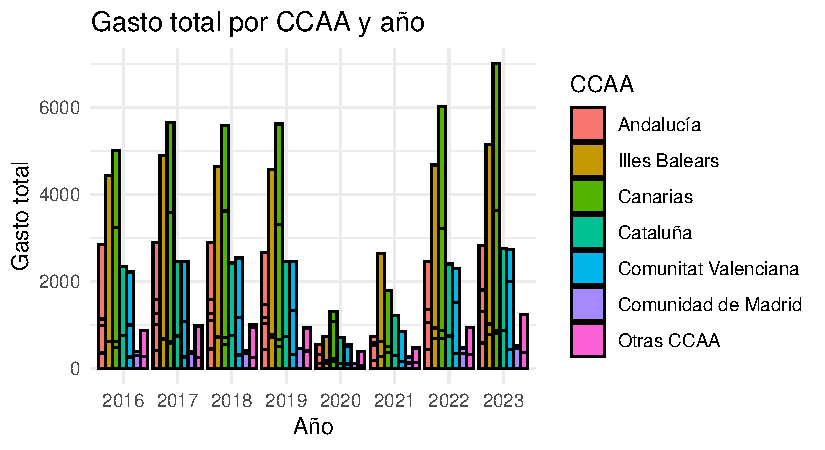
\includegraphics{ProyectoAED2024_Rmd_files/figure-latex/unnamed-chunk-22-1.pdf}

\begin{Shaded}
\begin{Highlighting}[]
\CommentTok{\# Nos centramos en un año en concreto y visualizamos el}
\CommentTok{\# gasto total por país en ese año}
\FunctionTok{ggplot}\NormalTok{(datos[datos}\SpecialCharTok{$}\NormalTok{Periodo }\SpecialCharTok{==} \DecValTok{2023}\NormalTok{, ], }\FunctionTok{aes}\NormalTok{(}\AttributeTok{x =} \FunctionTok{reorder}\NormalTok{(Pais,}
    \SpecialCharTok{{-}}\NormalTok{Gasto\_total), }\AttributeTok{y =}\NormalTok{ Gasto\_total)) }\SpecialCharTok{+} \FunctionTok{geom\_bar}\NormalTok{(}\AttributeTok{stat =} \StringTok{"identity"}\NormalTok{,}
    \FunctionTok{aes}\NormalTok{(}\AttributeTok{fill =}\NormalTok{ Pais)) }\SpecialCharTok{+} \FunctionTok{coord\_flip}\NormalTok{() }\SpecialCharTok{+} \FunctionTok{labs}\NormalTok{(}\AttributeTok{title =} \StringTok{"Gasto por país de residencia en 2023"}\NormalTok{,}
    \AttributeTok{x =} \StringTok{"Gasto total en millones de euros"}\NormalTok{, }\AttributeTok{y =} \StringTok{"País"}\NormalTok{) }\SpecialCharTok{+} \FunctionTok{theme}\NormalTok{(}\AttributeTok{legend.position =} \StringTok{"none"}\NormalTok{)}
\end{Highlighting}
\end{Shaded}

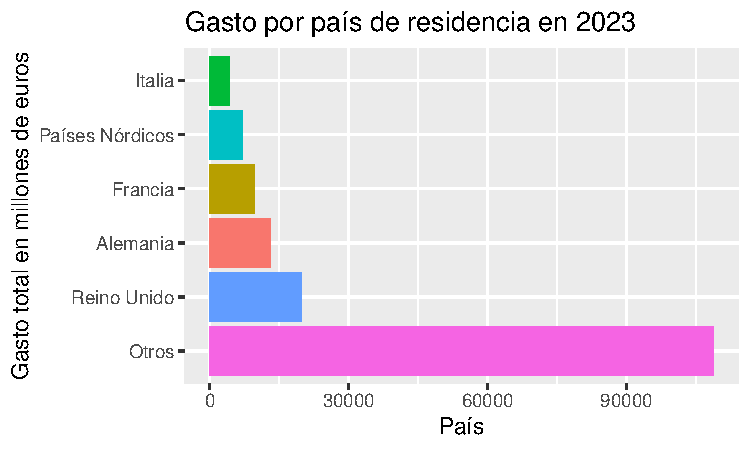
\includegraphics{ProyectoAED2024_Rmd_files/figure-latex/unnamed-chunk-22-2.pdf}

\begin{Shaded}
\begin{Highlighting}[]
\CommentTok{\# Para analizar únicamente una variable por país en una}
\CommentTok{\# sola Comunidad Autónoma.}
\FunctionTok{ggplot}\NormalTok{(datos, }\FunctionTok{aes}\NormalTok{(}\AttributeTok{x =}\NormalTok{ Pais, }\AttributeTok{y =}\NormalTok{ Duracion\_media)) }\SpecialCharTok{+} \FunctionTok{geom\_bar}\NormalTok{(}\AttributeTok{stat =} \StringTok{"identity"}\NormalTok{,}
    \AttributeTok{fill =} \StringTok{"red"}\NormalTok{) }\SpecialCharTok{+} \FunctionTok{facet\_grid}\NormalTok{(. }\SpecialCharTok{\textasciitilde{}}\NormalTok{ CCAA[}\StringTok{"i"}\NormalTok{], }\AttributeTok{scales =} \StringTok{"free"}\NormalTok{) }\SpecialCharTok{+}
    \FunctionTok{labs}\NormalTok{(}\AttributeTok{title =} \StringTok{"Duración media del viaje por país en Andalucía"}\NormalTok{,}
        \AttributeTok{x =} \StringTok{"País"}\NormalTok{, }\AttributeTok{y =} \StringTok{"Duración media del viaje"}\NormalTok{)}
\end{Highlighting}
\end{Shaded}

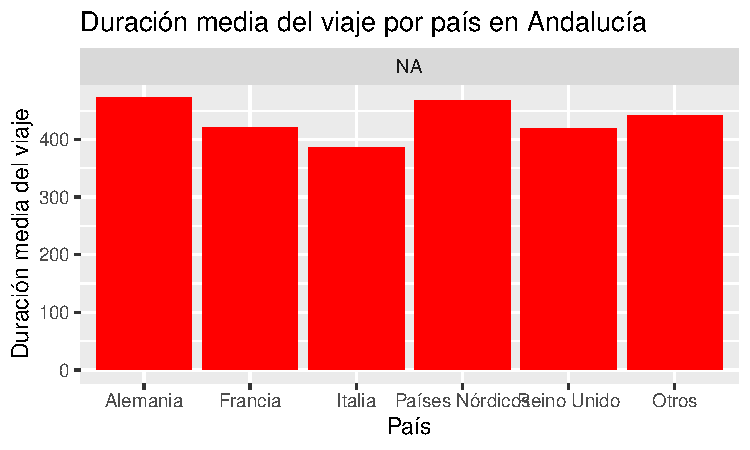
\includegraphics{ProyectoAED2024_Rmd_files/figure-latex/unnamed-chunk-22-3.pdf}

\begin{Shaded}
\begin{Highlighting}[]
\CommentTok{\# Para todas las Comunidades Autónomas por separado}
\FunctionTok{ggplot}\NormalTok{(datos, }\FunctionTok{aes}\NormalTok{(}\AttributeTok{x =}\NormalTok{ Pais, }\AttributeTok{y =}\NormalTok{ Duracion\_media)) }\SpecialCharTok{+} \FunctionTok{geom\_bar}\NormalTok{(}\AttributeTok{stat =} \StringTok{"identity"}\NormalTok{,}
    \AttributeTok{fill =} \StringTok{"purple"}\NormalTok{) }\SpecialCharTok{+} \FunctionTok{facet\_wrap}\NormalTok{(}\SpecialCharTok{\textasciitilde{}}\NormalTok{CCAA, }\AttributeTok{scales =} \StringTok{"free\_y"}\NormalTok{) }\SpecialCharTok{+}
    \FunctionTok{labs}\NormalTok{(}\AttributeTok{title =} \StringTok{"Duración media del viaje por país en cada Comunidad Autónoma"}\NormalTok{,}
        \AttributeTok{x =} \StringTok{"País"}\NormalTok{, }\AttributeTok{y =} \StringTok{"Duración media del viaje"}\NormalTok{) }\SpecialCharTok{+} \FunctionTok{theme}\NormalTok{(}\AttributeTok{axis.text.x =} \FunctionTok{element\_text}\NormalTok{(}\AttributeTok{angle =} \DecValTok{90}\NormalTok{,}
    \AttributeTok{hjust =} \DecValTok{1}\NormalTok{))}
\end{Highlighting}
\end{Shaded}

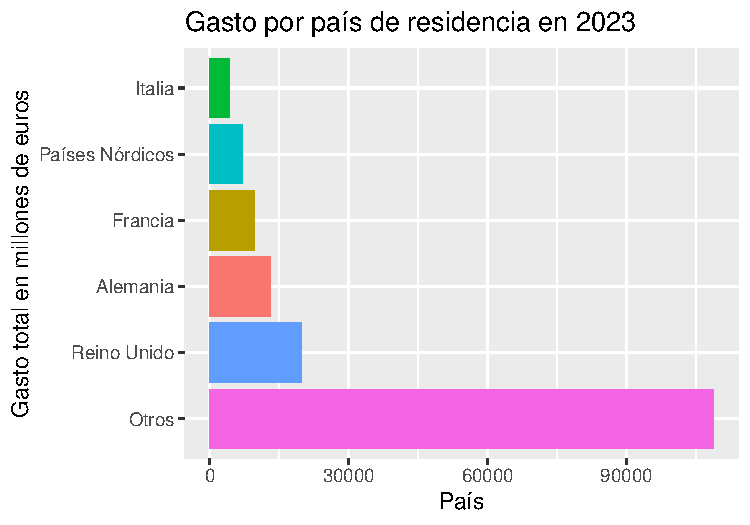
\includegraphics{ProyectoAED2024_Rmd_files/figure-latex/unnamed-chunk-23-1.pdf}

\section{Probamos a analizar el efecto del COVID en el gasto de los
turistas, así como los países que más reducieron su gasto debido a la
pandemia.}\label{probamos-a-analizar-el-efecto-del-covid-en-el-gasto-de-los-turistas-asuxed-como-los-pauxedses-que-muxe1s-reducieron-su-gasto-debido-a-la-pandemia.}

\begin{Shaded}
\begin{Highlighting}[]
\FunctionTok{library}\NormalTok{(tidyr)}

\NormalTok{covid }\OtherTok{\textless{}{-}}\NormalTok{ datos[datos}\SpecialCharTok{$}\NormalTok{Periodo }\SpecialCharTok{==} \DecValTok{2020}\NormalTok{, ]}
\NormalTok{no\_covid }\OtherTok{\textless{}{-}}\NormalTok{ datos[datos}\SpecialCharTok{$}\NormalTok{Periodo }\SpecialCharTok{!=} \DecValTok{2020}\NormalTok{, ]}
\NormalTok{media\_sin\_covid }\OtherTok{\textless{}{-}} \FunctionTok{mean}\NormalTok{(no\_covid}\SpecialCharTok{$}\NormalTok{Gasto\_total[])}
\NormalTok{media\_covid }\OtherTok{\textless{}{-}} \FunctionTok{mean}\NormalTok{(covid}\SpecialCharTok{$}\NormalTok{Gasto\_total)}
\FunctionTok{cat}\NormalTok{(}\StringTok{"La media del gasto total durante el COVID es de"}\NormalTok{, media\_covid,}
    \StringTok{"millones de euros}\SpecialCharTok{\textbackslash{}n}\StringTok{"}\NormalTok{)}
\end{Highlighting}
\end{Shaded}

\begin{verbatim}
## La media del gasto total durante el COVID es de 719.3212 millones de euros
\end{verbatim}

\begin{Shaded}
\begin{Highlighting}[]
\FunctionTok{cat}\NormalTok{(}\StringTok{"Mientras que sin COVID es de"}\NormalTok{, media\_sin\_covid, }\StringTok{"millones de euros}\SpecialCharTok{\textbackslash{}n}\StringTok{"}\NormalTok{)}
\end{Highlighting}
\end{Shaded}

\begin{verbatim}
## Mientras que sin COVID es de 2999.059 millones de euros
\end{verbatim}

\begin{Shaded}
\begin{Highlighting}[]
\NormalTok{datos }\SpecialCharTok{\%\textgreater{}\%}
    \FunctionTok{ggplot}\NormalTok{(}\FunctionTok{aes}\NormalTok{(}\AttributeTok{x =} \FunctionTok{factor}\NormalTok{(Periodo), }\AttributeTok{y =}\NormalTok{ Gasto\_total, }\AttributeTok{fill =}\NormalTok{ (Periodo }\SpecialCharTok{==}
        \DecValTok{2020}\NormalTok{))) }\SpecialCharTok{+} \FunctionTok{geom\_bar}\NormalTok{(}\AttributeTok{stat =} \StringTok{"identity"}\NormalTok{) }\SpecialCharTok{+} \FunctionTok{scale\_fill\_manual}\NormalTok{(}\AttributeTok{values =} \FunctionTok{c}\NormalTok{(}\StringTok{"grey"}\NormalTok{,}
    \StringTok{"red"}\NormalTok{)) }\SpecialCharTok{+} \FunctionTok{labs}\NormalTok{(}\AttributeTok{x =} \StringTok{"Año"}\NormalTok{, }\AttributeTok{y =} \StringTok{"Gasto Total de Turistas"}\NormalTok{,}
    \AttributeTok{title =} \StringTok{"Comparación del Gasto Total de Turistas por Año"}\NormalTok{) }\SpecialCharTok{+}
    \FunctionTok{theme\_minimal}\NormalTok{() }\SpecialCharTok{+} \FunctionTok{theme}\NormalTok{(}\AttributeTok{legend.position =} \StringTok{"none"}\NormalTok{)}
\end{Highlighting}
\end{Shaded}

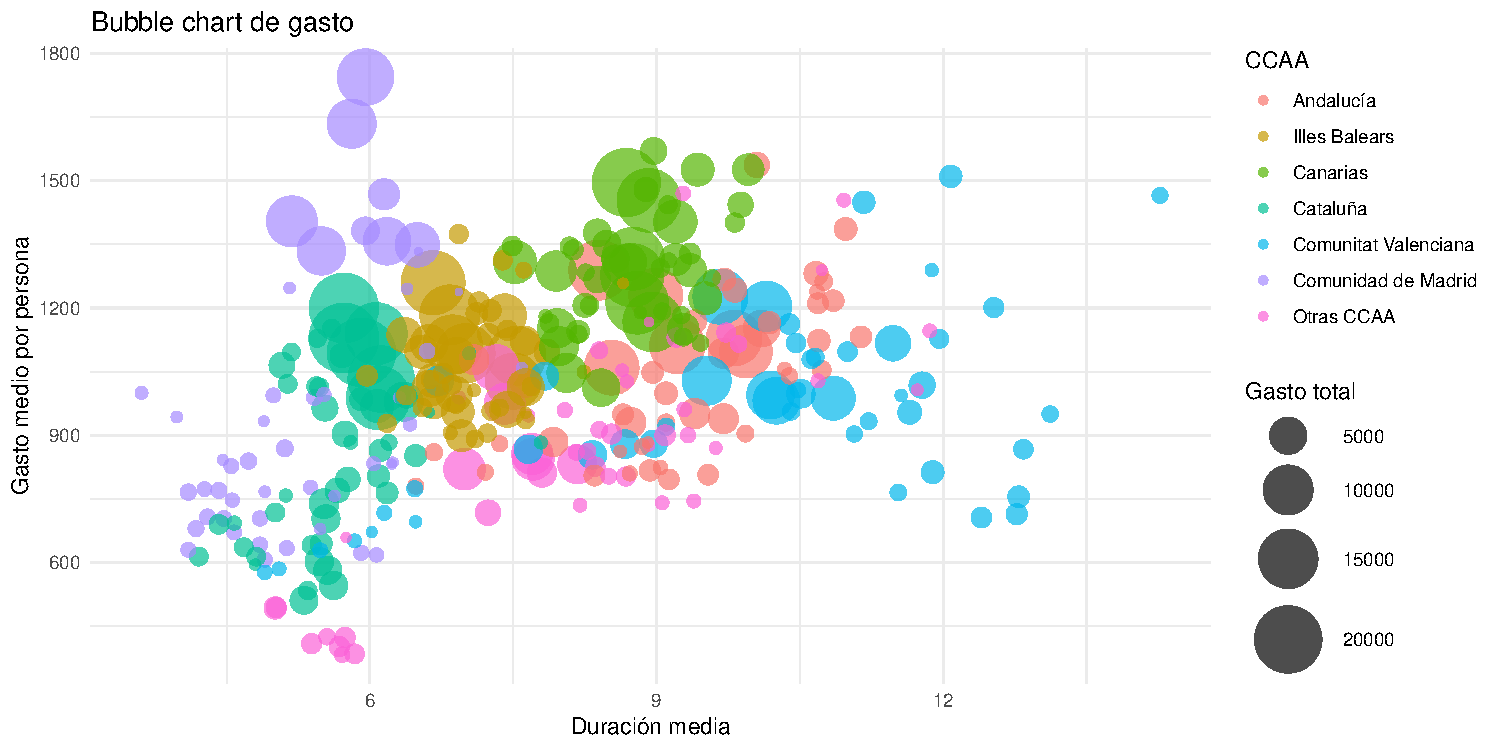
\includegraphics{ProyectoAED2024_Rmd_files/figure-latex/unnamed-chunk-24-1.pdf}

\begin{Shaded}
\begin{Highlighting}[]
\NormalTok{covid\_sin\_otros }\OtherTok{\textless{}{-}}\NormalTok{ covid[covid}\SpecialCharTok{$}\NormalTok{Pais }\SpecialCharTok{!=} \StringTok{"Otros"}\NormalTok{, ]  }\CommentTok{\# Elimino los datos correspondientes a otros países ya que son una suma y no se representa correctamente la tendencia.}
\NormalTok{covid\_sin\_otros }\SpecialCharTok{\%\textgreater{}\%}
    \FunctionTok{ggplot}\NormalTok{(}\FunctionTok{aes}\NormalTok{(}\AttributeTok{x =}\NormalTok{ Pais, }\AttributeTok{y =}\NormalTok{ Gasto\_total, }\AttributeTok{fill =}\NormalTok{ Pais)) }\SpecialCharTok{+} \FunctionTok{geom\_bar}\NormalTok{(}\AttributeTok{stat =} \StringTok{"identity"}\NormalTok{) }\SpecialCharTok{+}
    \FunctionTok{labs}\NormalTok{(}\AttributeTok{title =} \StringTok{"Gasto total de los distintos países durante el COVID"}\NormalTok{)  }\CommentTok{\# Reino Unido gastó más en COVID que el resto de países, Italia el que menos.}
\end{Highlighting}
\end{Shaded}

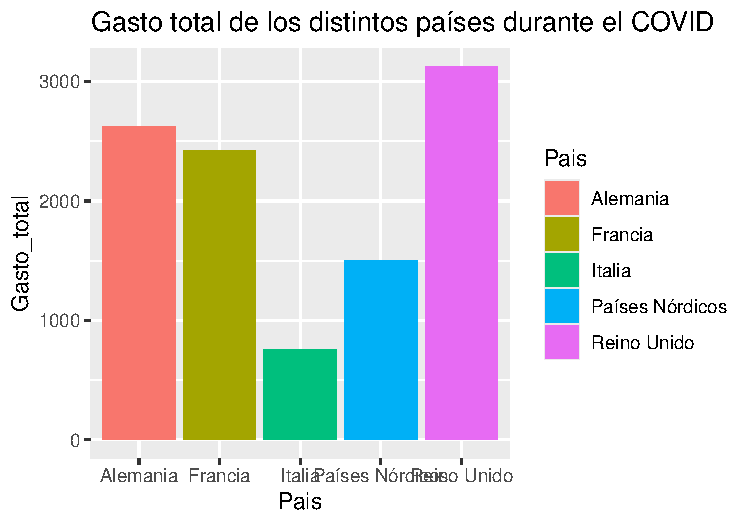
\includegraphics{ProyectoAED2024_Rmd_files/figure-latex/unnamed-chunk-24-2.pdf}

\begin{Shaded}
\begin{Highlighting}[]
\CommentTok{\# ¿En qué comunidad autónoma se viajó más durante el COVID?}
\NormalTok{covid\_sin\_otros }\SpecialCharTok{\%\textgreater{}\%}
    \FunctionTok{ggplot}\NormalTok{(}\FunctionTok{aes}\NormalTok{(}\AttributeTok{x =}\NormalTok{ CCAA, }\AttributeTok{y =}\NormalTok{ Gasto\_total, }\AttributeTok{fill =}\NormalTok{ CCAA)) }\SpecialCharTok{+} \FunctionTok{geom\_bar}\NormalTok{(}\AttributeTok{stat =} \StringTok{"identity"}\NormalTok{) }\SpecialCharTok{+}
    \FunctionTok{labs}\NormalTok{(}\AttributeTok{title =} \StringTok{"Gasto total en las distintas comunidades autónomas durante el COVID"}\NormalTok{)}
\end{Highlighting}
\end{Shaded}

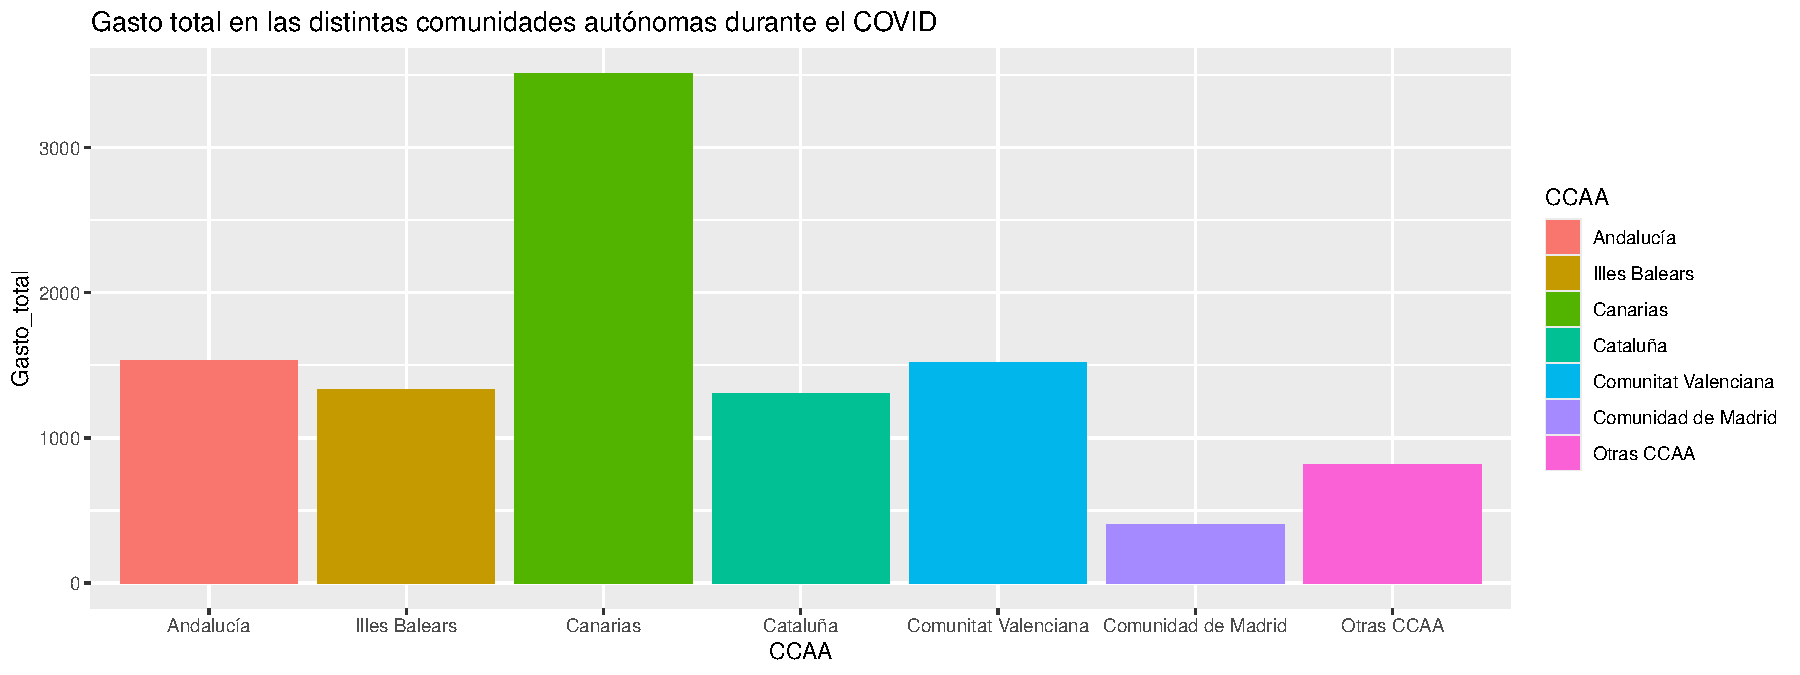
\includegraphics{ProyectoAED2024_Rmd_files/figure-latex/unnamed-chunk-25-1.pdf}

\begin{Shaded}
\begin{Highlighting}[]
\CommentTok{\# En Canarias el gasto de turistas fue mayor que en el}
\CommentTok{\# resto de Comunidades Autónomas durante el COVID, ¿menor}
\CommentTok{\# regulación?}
\end{Highlighting}
\end{Shaded}

Filtraremos los datos totales por el Periodo y recogeremos solo la
variable que nos sirve para representar la magnitud de valores en el
mapa de visualización, en este caso el gasto medio por persona

\begin{Shaded}
\begin{Highlighting}[]
\NormalTok{gastos\_medio\_residencia }\OtherTok{\textless{}{-}}\NormalTok{ datos\_total\_por\_residencia }\SpecialCharTok{\%\textgreater{}\%}
    \FunctionTok{select}\NormalTok{(Pais, Gasto\_medio\_persona, Periodo) }\SpecialCharTok{\%\textgreater{}\%}
    \FunctionTok{filter}\NormalTok{(Periodo }\SpecialCharTok{==} \StringTok{"2016"} \SpecialCharTok{\&}\NormalTok{ Pais }\SpecialCharTok{!=} \StringTok{"Total"}\NormalTok{)}

\NormalTok{gastos\_medio\_residencia\_PN }\OtherTok{\textless{}{-}}\NormalTok{ gastos\_medio\_residencia }\SpecialCharTok{\%\textgreater{}\%}
    \FunctionTok{select}\NormalTok{(Pais, Gasto\_medio\_persona, Periodo) }\SpecialCharTok{\%\textgreater{}\%}
    \FunctionTok{filter}\NormalTok{(Pais }\SpecialCharTok{==} \StringTok{"Países Nórdicos"}\NormalTok{)}

\CommentTok{\# Introducimos 4 filas iguales sobre los países nórdicos}
\CommentTok{\# para separar con el join estos y poder representarlos en}
\CommentTok{\# el mapa}

\NormalTok{gastos\_medio\_residencia }\OtherTok{\textless{}{-}} \FunctionTok{rbind}\NormalTok{(gastos\_medio\_residencia, gastos\_medio\_residencia\_PN,}
\NormalTok{    gastos\_medio\_residencia\_PN, gastos\_medio\_residencia\_PN, gastos\_medio\_residencia\_PN)}

\NormalTok{año\_ref }\OtherTok{\textless{}{-}} \DecValTok{2016}

\CommentTok{\# Datos}
\NormalTok{countries }\OtherTok{\textless{}{-}} \FunctionTok{gisco\_get\_countries}\NormalTok{(}\AttributeTok{year =}\NormalTok{ año\_ref, }\AttributeTok{resolution =} \DecValTok{20}\NormalTok{) }\SpecialCharTok{\%\textgreater{}\%}
    \FunctionTok{select}\NormalTok{(CNTR\_ID, NAME\_ENGL, geometry) }\SpecialCharTok{\%\textgreater{}\%}
    \FunctionTok{st\_transform}\NormalTok{(}\DecValTok{3035}\NormalTok{)}

\NormalTok{paises\_english }\OtherTok{\textless{}{-}} \FunctionTok{c}\NormalTok{(}\StringTok{"United Kingdom"}\NormalTok{, }\StringTok{"Denmark"}\NormalTok{, }\StringTok{"Germany"}\NormalTok{, }\StringTok{"France"}\NormalTok{,}
    \StringTok{"Italy"}\NormalTok{, }\StringTok{"Sweden"}\NormalTok{, }\StringTok{"Norway"}\NormalTok{, }\StringTok{"Iceland"}\NormalTok{, }\StringTok{"Finland"}\NormalTok{)}
\NormalTok{countries\_filtered }\OtherTok{\textless{}{-}}\NormalTok{ countries }\SpecialCharTok{\%\textgreater{}\%}
    \FunctionTok{filter}\NormalTok{(NAME\_ENGL }\SpecialCharTok{\%in\%}\NormalTok{ paises\_english)}

\CommentTok{\# Incluir columna de identificación de los países para unir}
\CommentTok{\# con las coordenadas de los mapas}

\NormalTok{CNTR\_ID }\OtherTok{\textless{}{-}} \FunctionTok{c}\NormalTok{(}\StringTok{"UK"}\NormalTok{, }\StringTok{"DK"}\NormalTok{, }\StringTok{"DE"}\NormalTok{, }\StringTok{"FR"}\NormalTok{, }\StringTok{"IT"}\NormalTok{, }\StringTok{"SE"}\NormalTok{, }\StringTok{"NO"}\NormalTok{, }\StringTok{"IS"}\NormalTok{,}
    \StringTok{"FI"}\NormalTok{)}
\NormalTok{gastos\_medio\_residencia }\OtherTok{\textless{}{-}} \FunctionTok{cbind}\NormalTok{(gastos\_medio\_residencia, CNTR\_ID)}


\NormalTok{gastos\_medio\_viz }\OtherTok{\textless{}{-}}\NormalTok{ gastos\_medio\_residencia }\SpecialCharTok{\%\textgreater{}\%}
    \FunctionTok{left\_join}\NormalTok{(countries, }\AttributeTok{by =} \FunctionTok{join\_by}\NormalTok{(CNTR\_ID }\SpecialCharTok{==}\NormalTok{ CNTR\_ID))}



\CommentTok{\# Mapa base}
\FunctionTok{ggplot}\NormalTok{(gastos\_medio\_viz) }\SpecialCharTok{+} \FunctionTok{geom\_sf}\NormalTok{(}\FunctionTok{aes}\NormalTok{(}\AttributeTok{geometry =}\NormalTok{ geometry, }\AttributeTok{fill =}\NormalTok{ Gasto\_medio\_persona)) }\SpecialCharTok{+}
    \FunctionTok{xlim}\NormalTok{(}\FunctionTok{c}\NormalTok{(}\DecValTok{2200000}\NormalTok{, }\DecValTok{7150000}\NormalTok{)) }\SpecialCharTok{+} \FunctionTok{ylim}\NormalTok{(}\FunctionTok{c}\NormalTok{(}\DecValTok{1380000}\NormalTok{, }\DecValTok{5500000}\NormalTok{))}
\end{Highlighting}
\end{Shaded}

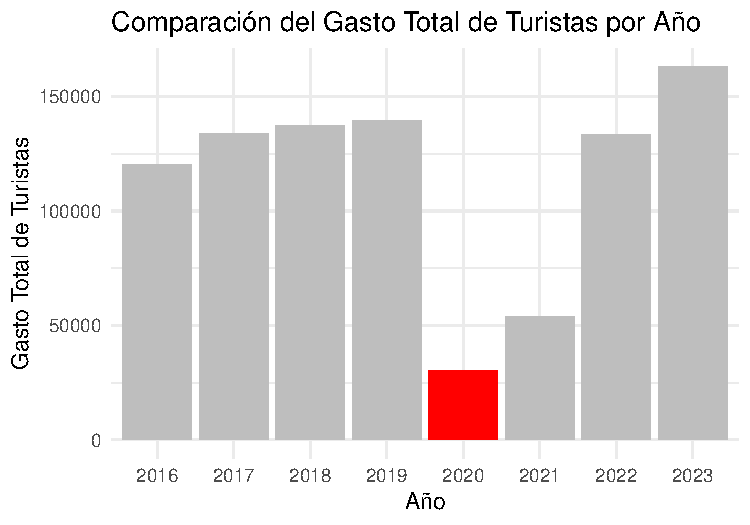
\includegraphics{ProyectoAED2024_Rmd_files/figure-latex/unnamed-chunk-26-1.pdf}

\begin{Shaded}
\begin{Highlighting}[]
\CommentTok{\# Marta: Te comenté esta parte porque me estaba dando}
\CommentTok{\# problemas al hacer knit no se por qué}

\CommentTok{\# Gráfico ggplot(gastos\_medio\_viz) + \# Primera capa con}
\CommentTok{\# todos los países geom\_sf(aes(geometry= geometry), data =}
\CommentTok{\# gastos\_medio\_viz, fill = \textquotesingle{}grey80\textquotesingle{}, color = NA) + \#}
\CommentTok{\# Establece límites xlim(c(2200000, 7150000)) +}
\CommentTok{\# ylim(c(1380000, 5500000))}
\end{Highlighting}
\end{Shaded}

\section{Búsqueda de relaciones entre variables
cuantitativas}\label{buxfasqueda-de-relaciones-entre-variables-cuantitativas}

Realizamos una visualización previa para detectar relaciones entre
variables cuantitativas. En el gráfico @ref(fig:correlaciones), se
observan 3 relaciones que podemos estudiar un poco más a fondo: el gasto
medio por persona frente al gasto medio diario, el gasto medio por
persona frente a la duración media y el gasto medio diario frente a la
duración media.

\begin{Shaded}
\begin{Highlighting}[]
\FunctionTok{library}\NormalTok{(GGally)  }\CommentTok{\# Librería para ggpairs}
\end{Highlighting}
\end{Shaded}

\begin{verbatim}
## Registered S3 method overwritten by 'GGally':
##   method from   
##   +.gg   ggplot2
\end{verbatim}

\begin{Shaded}
\begin{Highlighting}[]
\FunctionTok{ggpairs}\NormalTok{(datos[}\DecValTok{4}\SpecialCharTok{:}\DecValTok{7}\NormalTok{], }\AttributeTok{label =} \ConstantTok{FALSE}\NormalTok{) }\SpecialCharTok{+} \FunctionTok{theme}\NormalTok{(}\AttributeTok{axis.text =} \FunctionTok{element\_blank}\NormalTok{())  }\CommentTok{\# Quita los números de los ejes}
\end{Highlighting}
\end{Shaded}

\begin{verbatim}
## Warning in warn_if_args_exist(list(...)): Extra arguments: "label" are being
## ignored.  If these are meant to be aesthetics, submit them using the 'mapping'
## variable within ggpairs with ggplot2::aes or ggplot2::aes_string.
\end{verbatim}

\begin{figure}
\centering
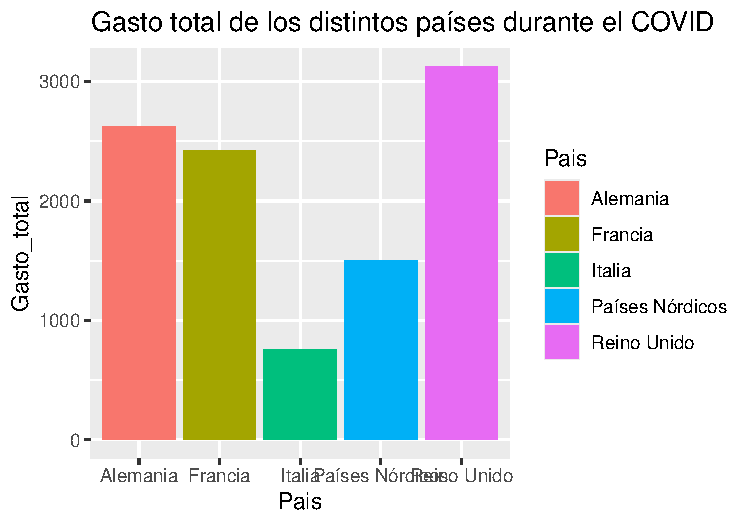
\includegraphics{ProyectoAED2024_Rmd_files/figure-latex/unnamed-chunk-27-1.pdf}
\caption{Gráficos de dispersión y correlaciones entre variables
cuantitativas}
\end{figure}

\begin{Shaded}
\begin{Highlighting}[]
\CommentTok{\# Gráficos de dispersión y correlaciones entre variables}
\CommentTok{\# cuantitativas}
\end{Highlighting}
\end{Shaded}

\subsection{Gasto medio por persona y duración
media}\label{gasto-medio-por-persona-y-duraciuxf3n-media}

\begin{Shaded}
\begin{Highlighting}[]
\CommentTok{\# Cálculo de las correlaciones}
\NormalTok{correlaciones }\OtherTok{\textless{}{-}}\NormalTok{ datos }\SpecialCharTok{\%\textgreater{}\%}
    \FunctionTok{group\_by}\NormalTok{(Pais) }\SpecialCharTok{\%\textgreater{}\%}
    \FunctionTok{summarise}\NormalTok{(}\AttributeTok{correlacion =} \FunctionTok{cor}\NormalTok{(Gasto\_medio\_persona, Duracion\_media))}


\FunctionTok{ggplot}\NormalTok{(}\AttributeTok{data =}\NormalTok{ datos, }\FunctionTok{aes}\NormalTok{(}\AttributeTok{x =}\NormalTok{ Gasto\_medio\_persona, }\AttributeTok{y =}\NormalTok{ Duracion\_media,}
    \AttributeTok{color =}\NormalTok{ CCAA)) }\SpecialCharTok{+} \FunctionTok{geom\_point}\NormalTok{() }\SpecialCharTok{+} \FunctionTok{facet\_wrap}\NormalTok{(}\SpecialCharTok{\textasciitilde{}}\NormalTok{Pais, }\AttributeTok{labeller =} \FunctionTok{label\_wrap\_gen}\NormalTok{(}\AttributeTok{width =} \DecValTok{15}\NormalTok{)) }\SpecialCharTok{+}
    \FunctionTok{labs}\NormalTok{(}\AttributeTok{title =} \StringTok{"Relación entre gasto medio por persona y duración media por país de residencia"}\NormalTok{,}
        \AttributeTok{x =} \StringTok{"Gasto medio por persona (euros)"}\NormalTok{, }\AttributeTok{y =} \StringTok{"Duración media de los viajes (días)"}\NormalTok{) }\SpecialCharTok{+}
    \FunctionTok{theme\_minimal}\NormalTok{() }\SpecialCharTok{+} \FunctionTok{geom\_text}\NormalTok{(}\AttributeTok{data =}\NormalTok{ correlaciones, }\FunctionTok{aes}\NormalTok{(}\AttributeTok{label =} \FunctionTok{paste}\NormalTok{(}\StringTok{"Cor.:"}\NormalTok{,}
    \FunctionTok{round}\NormalTok{(correlacion, }\DecValTok{2}\NormalTok{))), }\AttributeTok{x =} \ConstantTok{Inf}\NormalTok{, }\AttributeTok{y =} \ConstantTok{Inf}\NormalTok{, }\AttributeTok{hjust =} \FloatTok{1.5}\NormalTok{, }\AttributeTok{vjust =} \FloatTok{1.1}\NormalTok{,}
    \AttributeTok{size =} \DecValTok{3}\NormalTok{, }\AttributeTok{color =} \StringTok{"black"}\NormalTok{) }\SpecialCharTok{+} \FunctionTok{theme}\NormalTok{(}\AttributeTok{axis.text.x =} \FunctionTok{element\_blank}\NormalTok{())  }\CommentTok{\# Quita los números del eje X}
\end{Highlighting}
\end{Shaded}

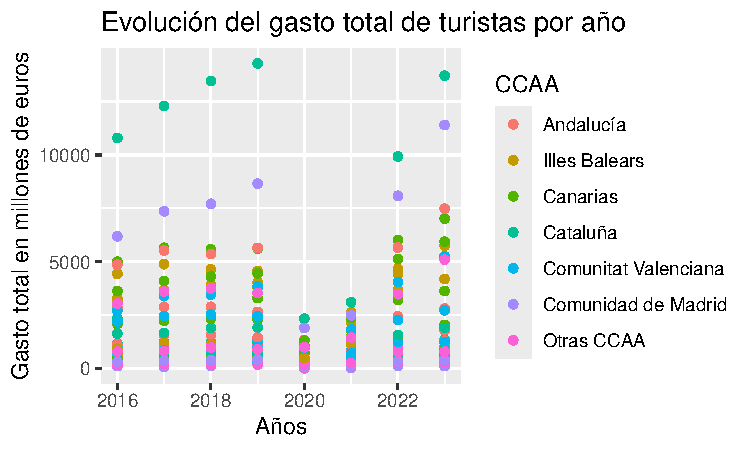
\includegraphics{ProyectoAED2024_Rmd_files/figure-latex/unnamed-chunk-28-1.pdf}

Se observa una relación aproximadamente lineal para la mayoría de
países, donde se distinguen claramente la tendendica de duración de los
viajes en las distintas comunidades autónomas, casi siempre mayor en la
Comunitat Valenciana (salvo en Italia, probablemente por cercanía),
excepto en Otros. Debido a que esta categoría engloba a el resto de
países del mundo, es más díficil encontara relaciones.

\subsection{Gasto medio por persona frente al gasto medio diario por
persona}\label{gasto-medio-por-persona-frente-al-gasto-medio-diario-por-persona}

Esta parece a priori la relación más obvia entre variables.

\begin{Shaded}
\begin{Highlighting}[]
\CommentTok{\# Cálculo de las correlaciones}
\NormalTok{correlaciones }\OtherTok{\textless{}{-}}\NormalTok{ datos }\SpecialCharTok{\%\textgreater{}\%}
    \FunctionTok{group\_by}\NormalTok{(CCAA) }\SpecialCharTok{\%\textgreater{}\%}
    \FunctionTok{summarise}\NormalTok{(}\AttributeTok{correlacion =} \FunctionTok{cor}\NormalTok{(Gasto\_medio\_persona, Gasto\_medio\_diario\_persona))}

\FunctionTok{ggplot}\NormalTok{(}\AttributeTok{data =}\NormalTok{ datos, }\FunctionTok{aes}\NormalTok{(}\AttributeTok{x =}\NormalTok{ Gasto\_medio\_persona, }\AttributeTok{y =}\NormalTok{ Gasto\_medio\_diario\_persona,}
    \AttributeTok{color =}\NormalTok{ Pais)) }\SpecialCharTok{+} \FunctionTok{geom\_point}\NormalTok{() }\SpecialCharTok{+} \FunctionTok{facet\_wrap}\NormalTok{(}\SpecialCharTok{\textasciitilde{}}\NormalTok{CCAA, }\AttributeTok{labeller =} \FunctionTok{label\_wrap\_gen}\NormalTok{(}\AttributeTok{width =} \DecValTok{15}\NormalTok{)) }\SpecialCharTok{+}
    \FunctionTok{labs}\NormalTok{(}\AttributeTok{title =} \StringTok{"Relación entre gasto medio por persona y gasto medio diario por comunidad autónoma"}\NormalTok{,}
        \AttributeTok{x =} \StringTok{"Gasto medio por persona (euros)"}\NormalTok{, }\AttributeTok{y =} \StringTok{"Gasto medio diario por persona (días)"}\NormalTok{) }\SpecialCharTok{+}
    \FunctionTok{theme\_minimal}\NormalTok{() }\SpecialCharTok{+} \FunctionTok{geom\_text}\NormalTok{(}\AttributeTok{data =}\NormalTok{ correlaciones, }\FunctionTok{aes}\NormalTok{(}\AttributeTok{label =} \FunctionTok{paste}\NormalTok{(}\StringTok{"Cor.:"}\NormalTok{,}
    \FunctionTok{round}\NormalTok{(correlacion, }\DecValTok{2}\NormalTok{))), }\AttributeTok{x =} \ConstantTok{Inf}\NormalTok{, }\AttributeTok{y =} \ConstantTok{Inf}\NormalTok{, }\AttributeTok{hjust =} \FloatTok{1.6}\NormalTok{, }\AttributeTok{vjust =} \DecValTok{1}\NormalTok{,}
    \AttributeTok{size =} \DecValTok{3}\NormalTok{, }\AttributeTok{color =} \StringTok{"black"}\NormalTok{) }\SpecialCharTok{+} \FunctionTok{theme}\NormalTok{(}\AttributeTok{axis.text.x =} \FunctionTok{element\_blank}\NormalTok{())  }\CommentTok{\# Quita los números del eje X}
\end{Highlighting}
\end{Shaded}

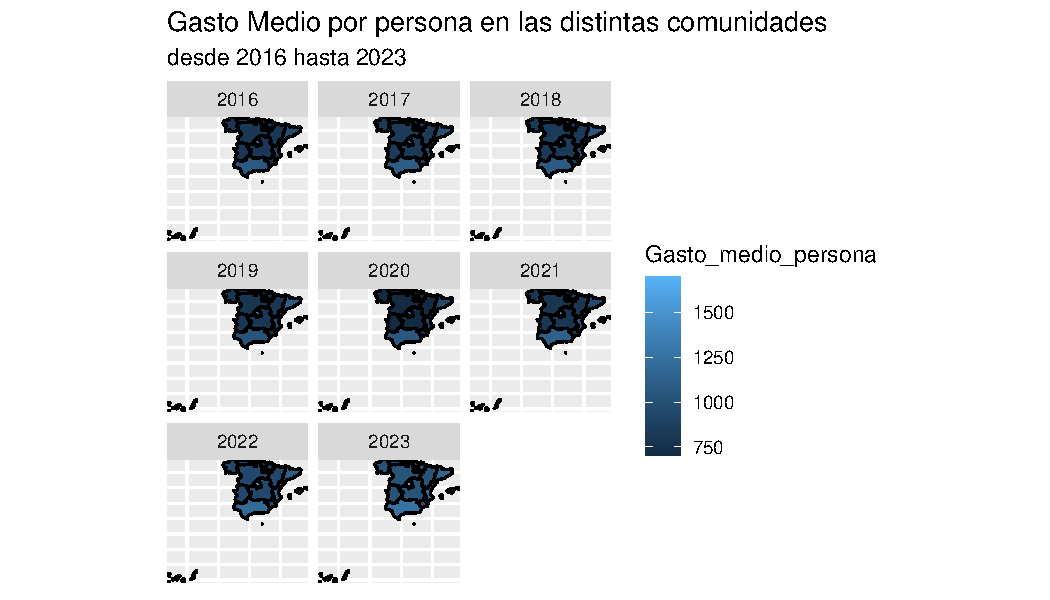
\includegraphics{ProyectoAED2024_Rmd_files/figure-latex/unnamed-chunk-29-1.pdf}
En la Comunitat Valenciana es donde hay una peor correlación, esto puede
estar relacionado con que es también el destino de mayor duración de los
viajes, lo que puede provocar un menor gasto medio diario.

\begin{Shaded}
\begin{Highlighting}[]
\FunctionTok{ggplot}\NormalTok{(}\AttributeTok{data =}\NormalTok{ datos, }\FunctionTok{aes}\NormalTok{(}\AttributeTok{x=}\NormalTok{Gasto\_medio\_persona, }\AttributeTok{y =}\NormalTok{Gasto\_medio\_diario\_persona, }\AttributeTok{color =}\NormalTok{ Duracion\_media)) }\SpecialCharTok{+} \FunctionTok{geom\_point}\NormalTok{(}\AttributeTok{size =} \DecValTok{2}\NormalTok{)  }\SpecialCharTok{+} \FunctionTok{scale\_color\_gradient}\NormalTok{(}\AttributeTok{low =} \StringTok{"lightgreen"}\NormalTok{, }\AttributeTok{high =} \StringTok{"darkgreen"}\NormalTok{) }\SpecialCharTok{+}  \CommentTok{\# Gradiente en tonos de verde}
  \FunctionTok{labs}\NormalTok{(}\AttributeTok{title =} \StringTok{"Relación entre gasto medio por persona y gasto medio diario por comunidad autónoma"}\NormalTok{,}
       \AttributeTok{x =} \StringTok{"Gasto medio por persona (euros)"}\NormalTok{,}
       \AttributeTok{y =} \StringTok{"Gasto medio diario por persona (días)"}\NormalTok{,}
       \AttributeTok{color =} \StringTok{"Duración media (días)"}\NormalTok{) }\SpecialCharTok{+} \FunctionTok{theme\_minimal}\NormalTok{() }
\end{Highlighting}
\end{Shaded}

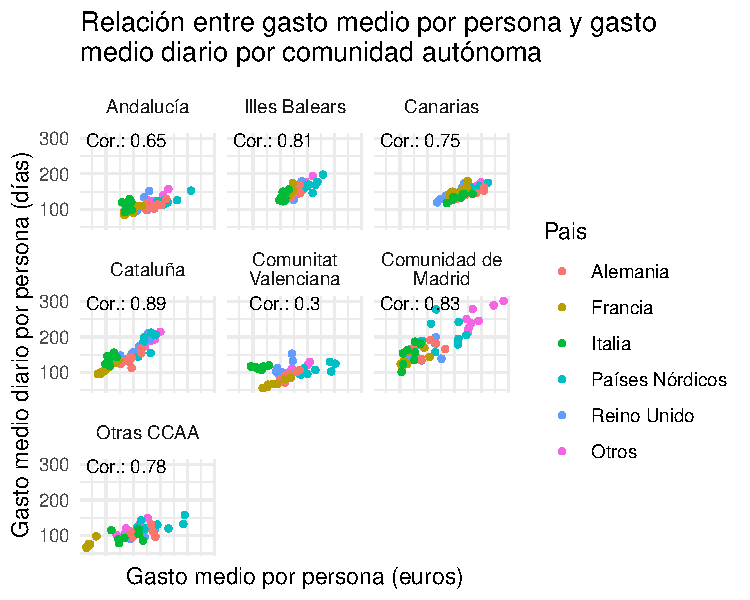
\includegraphics{ProyectoAED2024_Rmd_files/figure-latex/unnamed-chunk-30-1.pdf}
En el gráfico (referenciar) se puede ver que generalmente a mayor gasto
medio por persona también se produce un mayor gasto medio diario. Sin
embargo, observamos que aparentemente un aumento de la duración de los
viajes provoca una disminución del gasto medio diario. Vamos a
visualizar esto más claramente a continuación.

\subsection{Gasto medio diario y duracion
media}\label{gasto-medio-diario-y-duracion-media}

\begin{Shaded}
\begin{Highlighting}[]
\CommentTok{\# Cálculo de las correlaciones}
\NormalTok{correlaciones }\OtherTok{\textless{}{-}}\NormalTok{ datos }\SpecialCharTok{\%\textgreater{}\%}
    \FunctionTok{group\_by}\NormalTok{(Pais) }\SpecialCharTok{\%\textgreater{}\%}
    \FunctionTok{summarise}\NormalTok{(}\AttributeTok{correlacion =} \FunctionTok{cor}\NormalTok{(Gasto\_medio\_diario\_persona, Duracion\_media))}


\FunctionTok{ggplot}\NormalTok{(}\AttributeTok{data =}\NormalTok{ datos, }\FunctionTok{aes}\NormalTok{(}\AttributeTok{x =}\NormalTok{ Gasto\_medio\_diario\_persona, }\AttributeTok{y =}\NormalTok{ Duracion\_media,}
    \AttributeTok{color =}\NormalTok{ CCAA)) }\SpecialCharTok{+} \FunctionTok{geom\_point}\NormalTok{() }\SpecialCharTok{+} \FunctionTok{facet\_wrap}\NormalTok{(}\SpecialCharTok{\textasciitilde{}}\NormalTok{Pais, }\AttributeTok{labeller =} \FunctionTok{label\_wrap\_gen}\NormalTok{(}\AttributeTok{width =} \DecValTok{15}\NormalTok{)) }\SpecialCharTok{+}
    \FunctionTok{labs}\NormalTok{(}\AttributeTok{title =} \StringTok{"Relación entre gasto medio por persona y duración media por país de residencia"}\NormalTok{,}
        \AttributeTok{x =} \StringTok{"Gasto medio por persona (euros)"}\NormalTok{, }\AttributeTok{y =} \StringTok{"Duración media de los viajes (días)"}\NormalTok{) }\SpecialCharTok{+}
    \FunctionTok{theme\_minimal}\NormalTok{() }\SpecialCharTok{+} \FunctionTok{geom\_text}\NormalTok{(}\AttributeTok{data =}\NormalTok{ correlaciones, }\FunctionTok{aes}\NormalTok{(}\AttributeTok{label =} \FunctionTok{paste}\NormalTok{(}\StringTok{"Cor.:"}\NormalTok{,}
    \FunctionTok{round}\NormalTok{(correlacion, }\DecValTok{2}\NormalTok{))), }\AttributeTok{x =} \ConstantTok{Inf}\NormalTok{, }\AttributeTok{y =} \ConstantTok{Inf}\NormalTok{, }\AttributeTok{hjust =} \DecValTok{1}\NormalTok{, }\AttributeTok{vjust =} \DecValTok{1}\NormalTok{,}
    \AttributeTok{size =} \DecValTok{3}\NormalTok{, }\AttributeTok{color =} \StringTok{"black"}\NormalTok{)}
\end{Highlighting}
\end{Shaded}

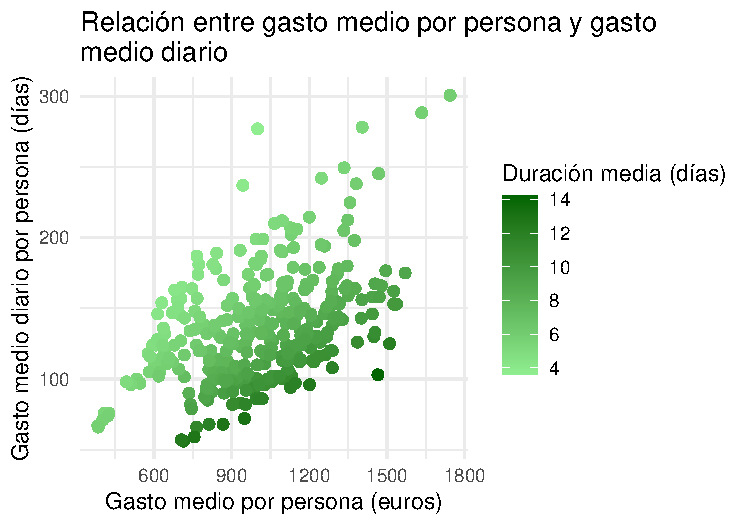
\includegraphics{ProyectoAED2024_Rmd_files/figure-latex/unnamed-chunk-31-1.pdf}
Ahora podemos observar de manera clara que a mayor duración de los
viajes se produce un menor gasto medio por persona.

%%%%%%%%%%%%%%%%%%%%%%%%%%%%%%%%%%%%%%%%%%

\vspace{6pt}

%%%%%%%%%%%%%%%%%%%%%%%%%%%%%%%%%%%%%%%%%%
%% optional

% Only for the journal Methods and Protocols:
% If you wish to submit a video article, please do so with any other supplementary material.
% \supplementary{The following supporting information can be downloaded at: \linksupplementary{s1}, Figure S1: title; Table S1: title; Video S1: title. A supporting video article is available at doi: link.}

%%%%%%%%%%%%%%%%%%%%%%%%%%%%%%%%%%%%%%%%%%







%%%%%%%%%%%%%%%%%%%%%%%%%%%%%%%%%%%%%%%%%%
%% Optional

%% Only for journal Encyclopedia


%%%%%%%%%%%%%%%%%%%%%%%%%%%%%%%%%%%%%%%%%%
%% Optional
\input{"appendix.tex"}
%%%%%%%%%%%%%%%%%%%%%%%%%%%%%%%%%%%%%%%%%%
\begin{adjustwidth}{-\extralength}{0cm}

%\printendnotes[custom] % Un-comment to print a list of endnotes


\reftitle{References}
\bibliography{mybibfile.bib}

% If authors have biography, please use the format below
%\section*{Short Biography of Authors}
%\bio
%{\raisebox{-0.35cm}{\includegraphics[width=3.5cm,height=5.3cm,clip,keepaspectratio]{Definitions/author1.pdf}}}
%{\textbf{Firstname Lastname} Biography of first author}
%
%\bio
%{\raisebox{-0.35cm}{\includegraphics[width=3.5cm,height=5.3cm,clip,keepaspectratio]{Definitions/author2.jpg}}}
%{\textbf{Firstname Lastname} Biography of second author}

%%%%%%%%%%%%%%%%%%%%%%%%%%%%%%%%%%%%%%%%%%
%% for journal Sci
%\reviewreports{\\
%Reviewer 1 comments and authors’ response\\
%Reviewer 2 comments and authors’ response\\
%Reviewer 3 comments and authors’ response
%}
%%%%%%%%%%%%%%%%%%%%%%%%%%%%%%%%%%%%%%%%%%
\PublishersNote{}
\end{adjustwidth}


\end{document}
